%!TEX root = ../Bachelorarbeit.tex
\chapter{Data Centric Design}
\label{sec:dcd}
In diesem Kapitel wird die grundlegende Architektur der Anbindung eines persistenten Speichers im Core von Project-Zoom näher erläutert. Dieser Befindet sich im \tete{Common} Subprojekt im Paket \tete{projectZoom.core} und \tete{models}. Das gewählte Design hat vorrangig Auswirkungen auf die Art und Weise wie der Code für Datenmodelle geschrieben wird, erstreckt sich aber als Betrachtungsweise über die gesamte Architektur.

\section{Motivation}
\label{sec:dcdmotivation}
Das JSON Coast-To-Coast Design als Umsetzung des Data Centric Designs ist erstmals zusammenhängend und beispielunterlegt dargestellt wurden durch Pascal Voitet in seinem Blog Mandubian \cite{jctc}. Voitet ist selbst Mitwirkender am open Source Projekt Play und aktiver Scala Bibliotheken Autor (\tete{play-reactivemongo}\footnote{\url{ https://github.com/zenexity/Play-ReactiveMongo}}, \tete{play-autosource}\footnote{\url{ https://github.com/mandubian/play-autosource}}). 

Ein Webapplikation Backend ist zunehmend eine Verbindung zwischen verschiedenen anderen Backends und Frontends. Diese Entwicklung geht auf die Bereitstellung von APIs für viele große und kleine im Web verfügbare Dienste zurück. Anwendungen, welche Daten vorrangig aus anderen Quellen aggregieren, sind zum großen Teil mit der Datenmanipulation beschäftigt. Hier bietet sich ein Data Centric Design an. Für das Design grundlegend sind drei Entwicklungen. Zum einen das Aufstreben von NoSQL Datenbanken und zum anderen asynchrone Datenbanktreiber mit einfachen Methoden zur JSON Manipulation.

\subsection{NoSQL}
Die Entwicklung der Datenbank Management Systeme bestand viele Jahre lang in der Optimierung und Verbesserung bestehender relationaler Datenbank Modelle. Im Jahr 1998 kam dann der Term Not-only SQL (NoSQL) auf \cite{storage-solutions}. Heute gibt es verschiedene etablierte Datenbanken die keine reinen SQL Datenbanken mehr sind, bekannte Beispiele sind MongoDB, CouchDB, Apache Cassandra. MongoDB ist eine Open-Source Datenbank, welche ihre Daten Dokumenten basiert speichert.

\subsection{Datenbanktreiber}
Für die Anbindung von relationalen Datenbanken gibt es in Java die Java Database Connectivity (JDBC) Schnittstelle. Diese abstrahiert über Datenbanken und deren Treiber indem eine einheitliche API angeboten wird. Ausgerichtet ist JDBC auf relationale Datenbanken.

Um NoSQL Datenbanken anzubinden benötigt man, wie bei JDBC, einen eigenen Treiber. Der Unterschied ist, das es hier keine Abstraktionsebene über verschiedene NoSQL Datenbanken gibt. Dies liegt vorrangig an der sich stark unterscheidenden Struktur der einzelnen Speichersysteme. Die unterschiedlichen NoSQL Datenbanken sind jeweils speziell auf eine bestimmte Aufgabe ausgerichtet, wie z.B. Durchsatz, Verteilte Umgebungen oder Flexible Daten Schemas. 

\tete{ReactiveMongo} ist ein asynchroner Datenbanktreiber für MongoDB und die Programmiersprache Scala. Die Vorteile eines asynchronen Treibers liegen auf der Hand: Für jede synchrone Datenbank Abfrage wird normalerweise ein Thread verwendet, der bis zur Antwort blockiert ist. Bei mehreren Datenbankabfragen pro Request werden bei Last viele Threads benötigt um Datenbank abfragen auszuführen. Asynchrone Treiber umgehen dieses Problem indem sie Threads, welche Datenbank Abfragen ausführen, nicht blockieren. Für dieses Konzept ist es Notwendig Platzhalter einzuführen. Diese ersetzen das Ergebnis solange es noch nicht vorhanden ist.

\begin{lstlisting}[caption=Funktionssignatur für asynchronen Datenbankzugriff]
def findOneById(bid: BSONObjectID): Future[Option[Graph]]
\end{lstlisting}
 
Im Beispiel XXX zeigt die Funktionssignatur den Rückgabetyp \tete{Future[Option[Graph]]}. \tete{Future} ist hierbei genau dieser Platzhalter für ein Ergebnis welches noch nicht existiert. Arbeiten kann man mit einem \tete{Future} durch das Festlegen von Callbacks.


\subsection{Manipulation von JSON}
Das Data Centric Design basiert auf der Idee der direkten Manipulation von Daten. Für eine Umsetzung des Data Centric Designs mit Hilfe von JSON benötigt man somit eine Bibliothek, welche die Möglichkeit bietet, JSON zu transformieren und zu validieren.
 
Ein Beispiel für solch eine Bibliothek ist Play-JSON. Sie erlaubt das Validieren, Transformieren und Serialisieren. Ein Beispiel ist im Quelltextauszug \ref{lst:jsonbsp} zu sehen. Dort wird ein JSON Objekt erzeugt, welches anschließend zuerst Transformiert wird indem das Attribut \tete{role} angehangen wird und danach Validiert wird. Bei der Validierung wird überprüft ob der User über 18 Jahre alt ist.

\lstinputlisting[caption=Play JSON Transformations / Validierungs Beispiel, label=lst:jsonbsp, language=scala]{code/json_example.scala}

\section{Idee hinter Data Centric Design}
Das Ziel im Data Centric Design ist die direkte Manipulation von Daten. Der Fokus des Designs liegt auf der Daten Manipulation und dem Datenfluss. Wie bereits in \ref{sec:dcdmotivation} beschrieben, sind Webapplikation Backends immer Häufiger Knotenpunkte in einem mehrere Server durchlaufenden Datenfluss. Ein Teil dieses Datenflusses ist die Kommunikation des Backends mit der Datenbank und dem Client \ref{fig:dataflow}. 

\begin{figure}[h]   
  \centering     
  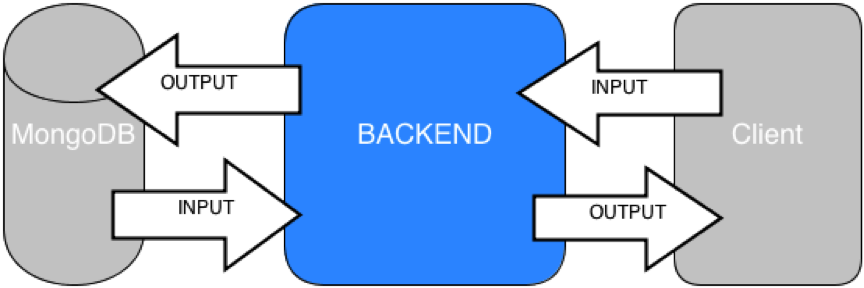
\includegraphics[width=0.8\textwidth]{img/dataflow.png}  
   \caption{Datenfluss zwischen Datenbank, Backend und Client}   
  \label{fig:dataflow} 
\end{figure}

In diesem Datenfluss soll es keine implizite Umwandlung der Daten in Objekte der Programmiersprache geben. Für ein einfaches durchleiten der Daten aus der Datenbank zum Client oder von einer anderen Webressource zum Client eine Umwandlung nicht notwendig und sinnvoll ist. 

Eine Deserialisierung der Daten in Objekte ist für komplizierte Business Logik von Vorteil. Statische Daten Modelle sollten immer dann verwendet werden, wenn die Manipulation der Daten kompliziert wird oder wenn die Verwendung externer Bibliotheken eine Objekt Repräsentation benötigt. 

Nach Voitot ist die Frage also nicht, statische Daten Modelle zu vergessen, sondern sie nur dann zu benutzen, wenn sie notwendig sind. Einfache und dynamische Strukturen sollten so oft es geht erhalten bleiben \cite{jctc}.

\section{Abgrenzung zum Objektrelationalen Abbildung}
Das Object-relational Mapping (ORM) bezeichnet man auch als All-Model-Approach. Hierbei erfolgt die Kommunikation mit der Datenbankschnittstelle über Objekte der Programmiersprache. Abfragen an die Datenbank resultieren in Objekten der Programmiersprache. Der Fokus der Objektrelationalen Abbildung liegt in der Überführung von Objekten der Objektorientierten Programmierung in ein relationales, tabellenorientiertes Schema \cite{wambler}. 

\begin{figure}[h]   
  \centering     
  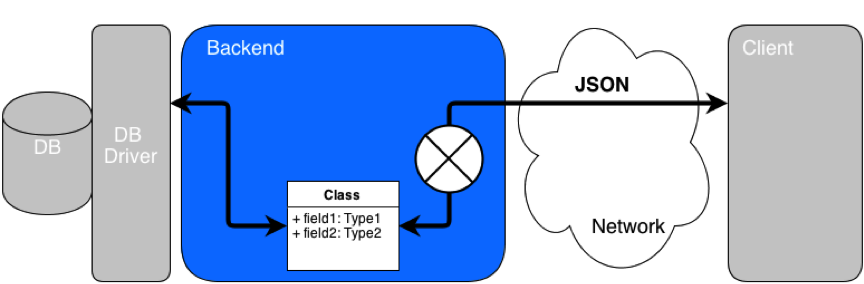
\includegraphics[width=0.8\textwidth]{img/orm.png}  
   \caption{Datenfluss einer Applikation bei Verwendung eines ORM Frameworks}   
  \label{fig:orm} 
\end{figure}

Der Hauptvorteil eines ORM liegt in der Abstraktion von der Datenbank. Für die Business Logik gibt es keinen Unterschied zwischen Objekten aus der Datenbank und Objekten der Programmiersprache. Die Datenbank kann meist ohne Änderungen an der Applikation ausgetauscht werden.

\FloatBarrier
\subsection{Objektrelationale Unverträglichkeit}

Ein ORM bringt einige konzeptionelle Probleme mit sich. Diese werden im allgemeinen in der Literatur als \tete{Object-relational Impedance Mismatch} (ORIM) bezeichnet. Die objektrelationale Unverträglichkeit resultiert aus den Unterschieden im zugrunde liegenden Konzept, sowie Differenzen in der Darstellung und den Erwartungen des Entwicklers \cite{bowers}.

Folgende Herausforderungen ergeben sich für die praktische Arbeit mit einem ORM:

\begin{itemize}
  \item Die Abbildung der Relationen zwischen den Objekten ist komplex. Es müssen One-to-One, One-to-Many und Many-to-Many Abhängikeiten ins Relationale Schema übertragen werden.
\item Ein weiterer wichtiger Punkt ist die Abbildung von Hierarchien und Vererbungen aus der Objekt Orientierten Programmierung in das physische Daten Modell. 
\item Innerhalb des ORM muss es ein Objekt Caching geben. Dieses ist notwendig um die Illusion zu erzeugen, dass es sich um ein Objekt der Programmiersprache handelt. Denn wird ein Objekt mehrmals aus der Datenbank abgefragt, so muss ein referenz-gleiches Objekt zurückgegeben werden \cite{inappropriate-abstractions}.
\item Der Entwickler muss die ORM Limitierungen die sich aus dem ORIM ergeben akzeptieren. Die Probleme müssen bekannt sein, um sie bereits bei der Daten Modellierung zu umgehen \cite{vietnam}. 
\end{itemize}

Ted Neward, Autor von „The Busy Java Developers Guide to Scala“, macht den frühen Erfolg von ORMs und die Erleichterungen, welche die ersten ORMs mit sich brachten, dafür verantwortlich, dass ORMs verwendet werden ohne deren Limitationen zu beachten. So kommt es zu Mehraufwand an Zeit und Energie für die Erhaltung und Anpassung an alle Nutzungsfälle \cite{vietnam}.

\subsection{Unterschiede zum Data Centric Design}
Das Data Centric Design ist viel stärker an die Datenbank gebunden und deren Austausch ist deutlich schwieriger. Dies sorgt aber dafür, dass keine Illusion einer abstrahierten Datenbank entsteht. Da das Data Centric Design ein Ansatz mit funktionalem Hintergrund ist, sind die Datenstrukturen in der Regel unveränderbar. Ein Caching zur Sicherung der Objektidendität ist daher nicht notwendig. Die Objektgleichheit ist in diesem Fall über Wertgleichheit definiert (vgl. Scala Case Klassen \cite{scala-case-class}). Im Gegensatz zum ORM muss der Entwickler sich beim Data Centric Design selbst um die Darstellung und Umwandlung seiner Daten in das Datenbank Format kümmern. Durch die Verwendung einer objekt- oder dokumentenbasierten Datenbank ist diese Umwandlung einfacher und mit weniger Problemen behaftet als eine Konvertierung in ein relationales Schema.

\section{Abgrenzung zu Data Access Objekt}
Implementierungen eines \tete{Data Access Object} (DAO, oft auch \tete{Data Access Procedure}) basiert auf dem \tete{Data Access Object} Pattern \cite{j2ee-pattern}.  Das Pattern hat das Ziel, den Datenzugriff und die Datenmanipulation in einen separaten Layer auszulagern. Es ergibt sich eine Kapselung der Datenbankzugriffe an einem Ort der Applikation. Bei der Umsetzung gibt es se Möglichkeit ein DAO zur Abstraktion der Datenbank als ganzes zu verwenden oder für jede einzelne Datenbankstruktur ein DAO anzulegen.

Der Hauptfokus liegt in der Abstrahierung der Datenbank. Bei Änderungen an der Datenquelle müssen in der Regel nur die Data Access Objects angepasst werden, der Anwendungscode bleibt in der Regel unberührt. Die Aufgabe der Serialisierung der Daten von den Strukturen der Anwendung in Strukturen der Datenbank sind nicht Aufgabe des DAO sondern des Data Transfer Object (DTO) \footnote{vgl. J2EE Patterns – Data Transfer Object \url{http://www.oracle.com/technetwork/java/transferobject-139757.html}}.

Im DAO findet über einen Datenbank Treiber direkter Zugriff auf die Datenbank statt. Man kann dieses Objekt somit als Mittelsmann zwischen Datenbank und Applikation sehen. Durch die direkte Kommunikation mit der Datenquelle können alle unterstützten Funktionen ausgenutzt werden. 

\subsection{Unterschiede zum Data Centric Design}


